\chapter{Verifica e validazione}
\label{cap:verifica-validazione}

Il seguente capitolo ha lo scopo di mostrare le tecniche di verifica e validazione del progetto, secondo le linee guida apprese durante il corso di Ingegneria del Software. \\
Verificare un prodotto ha l'obiettivo di controllare se l'introduzione di nuovi elementi nel codice ha generato dei problemi e se rispetta i requisiti designati. 
\\La validazione serve ad approvare il progetto qualora soddisfi tutti i requisiti imposti.

\section{Processo di Verifica}
Il processo di verifica è stato attuato durante tutto lo sviluppo del progetto per verificare le nuove funzionalità e comportamenti introdotti.\\
L'approccio all'introduzione di nuovi elementi con le relative funzioni è stato costantemente controllato da \textit{Roberto Martina}, responsabile di stage. Infatti  la tecnica più efficiente per lo sviluppo dell'applicazione è stata codificare una parte di webapp alla volta, verificare che il codice appena introdotto funzionasse correttamente nel suo insieme e soltanto dopo collegarlo alle altri parti di codice già sviluppate.\\
Quindi non si procedeva per codificare il "tutto" perché i requisiti potevano risultare non soddisfatti, comportando  il rischio di perdere l'obiettivo durante lo sviluppo. È stato seguito un approccio rigoroso, suddividendo il processo in passi distinti e verificando accuratamente la correttezza di ciascuno di essi.

\subsection{Debugging}
Una delle tecniche per verificare il giusto funzionamento dell'applicazione è stato il \textit{\textbf{Debugging}}. Effettuare il debug significava controllare a \textit{run-time} come si comportava l'applicazione durante l'interazione con l'utente. Dopo aver introdotto una nuova funzione per l'applicazione, si poteva effettuare il debug per verificare che la funzione introdotta agiva nel corretto modo e non introduceva nuovi problemi per gli altri elementi della webapp. \\
Lo strumento di \textit{debug} utilizzato per verificare il progetto è stato quello messo a disposizione da \textbf{IDE Eclipse}. \textit{Eclipse} fornisce sia il \textit{debug} del codice, ma anche il \textit{debug} per il server su cui viene eseguita la webapp.
Una feature di questo \textit{IDE} è l'introduzione dei \textit{breakpoint}, che consente di esaminare il codice linea per linea.\\ Posizionando un \textit{breakpoint} su una riga, l'applicazione si fermerà in corrispondenza di quel punto durante la sua esecuzione, consentendo al programmatore di avanzare passo dopo passo utilizzando i tasti \textit{F9, F10, F11, F12} al fine di individuare con precisione la potenziale fonte dell'errore.

\begin{figure}[H]
\bigskip
    \centering 
    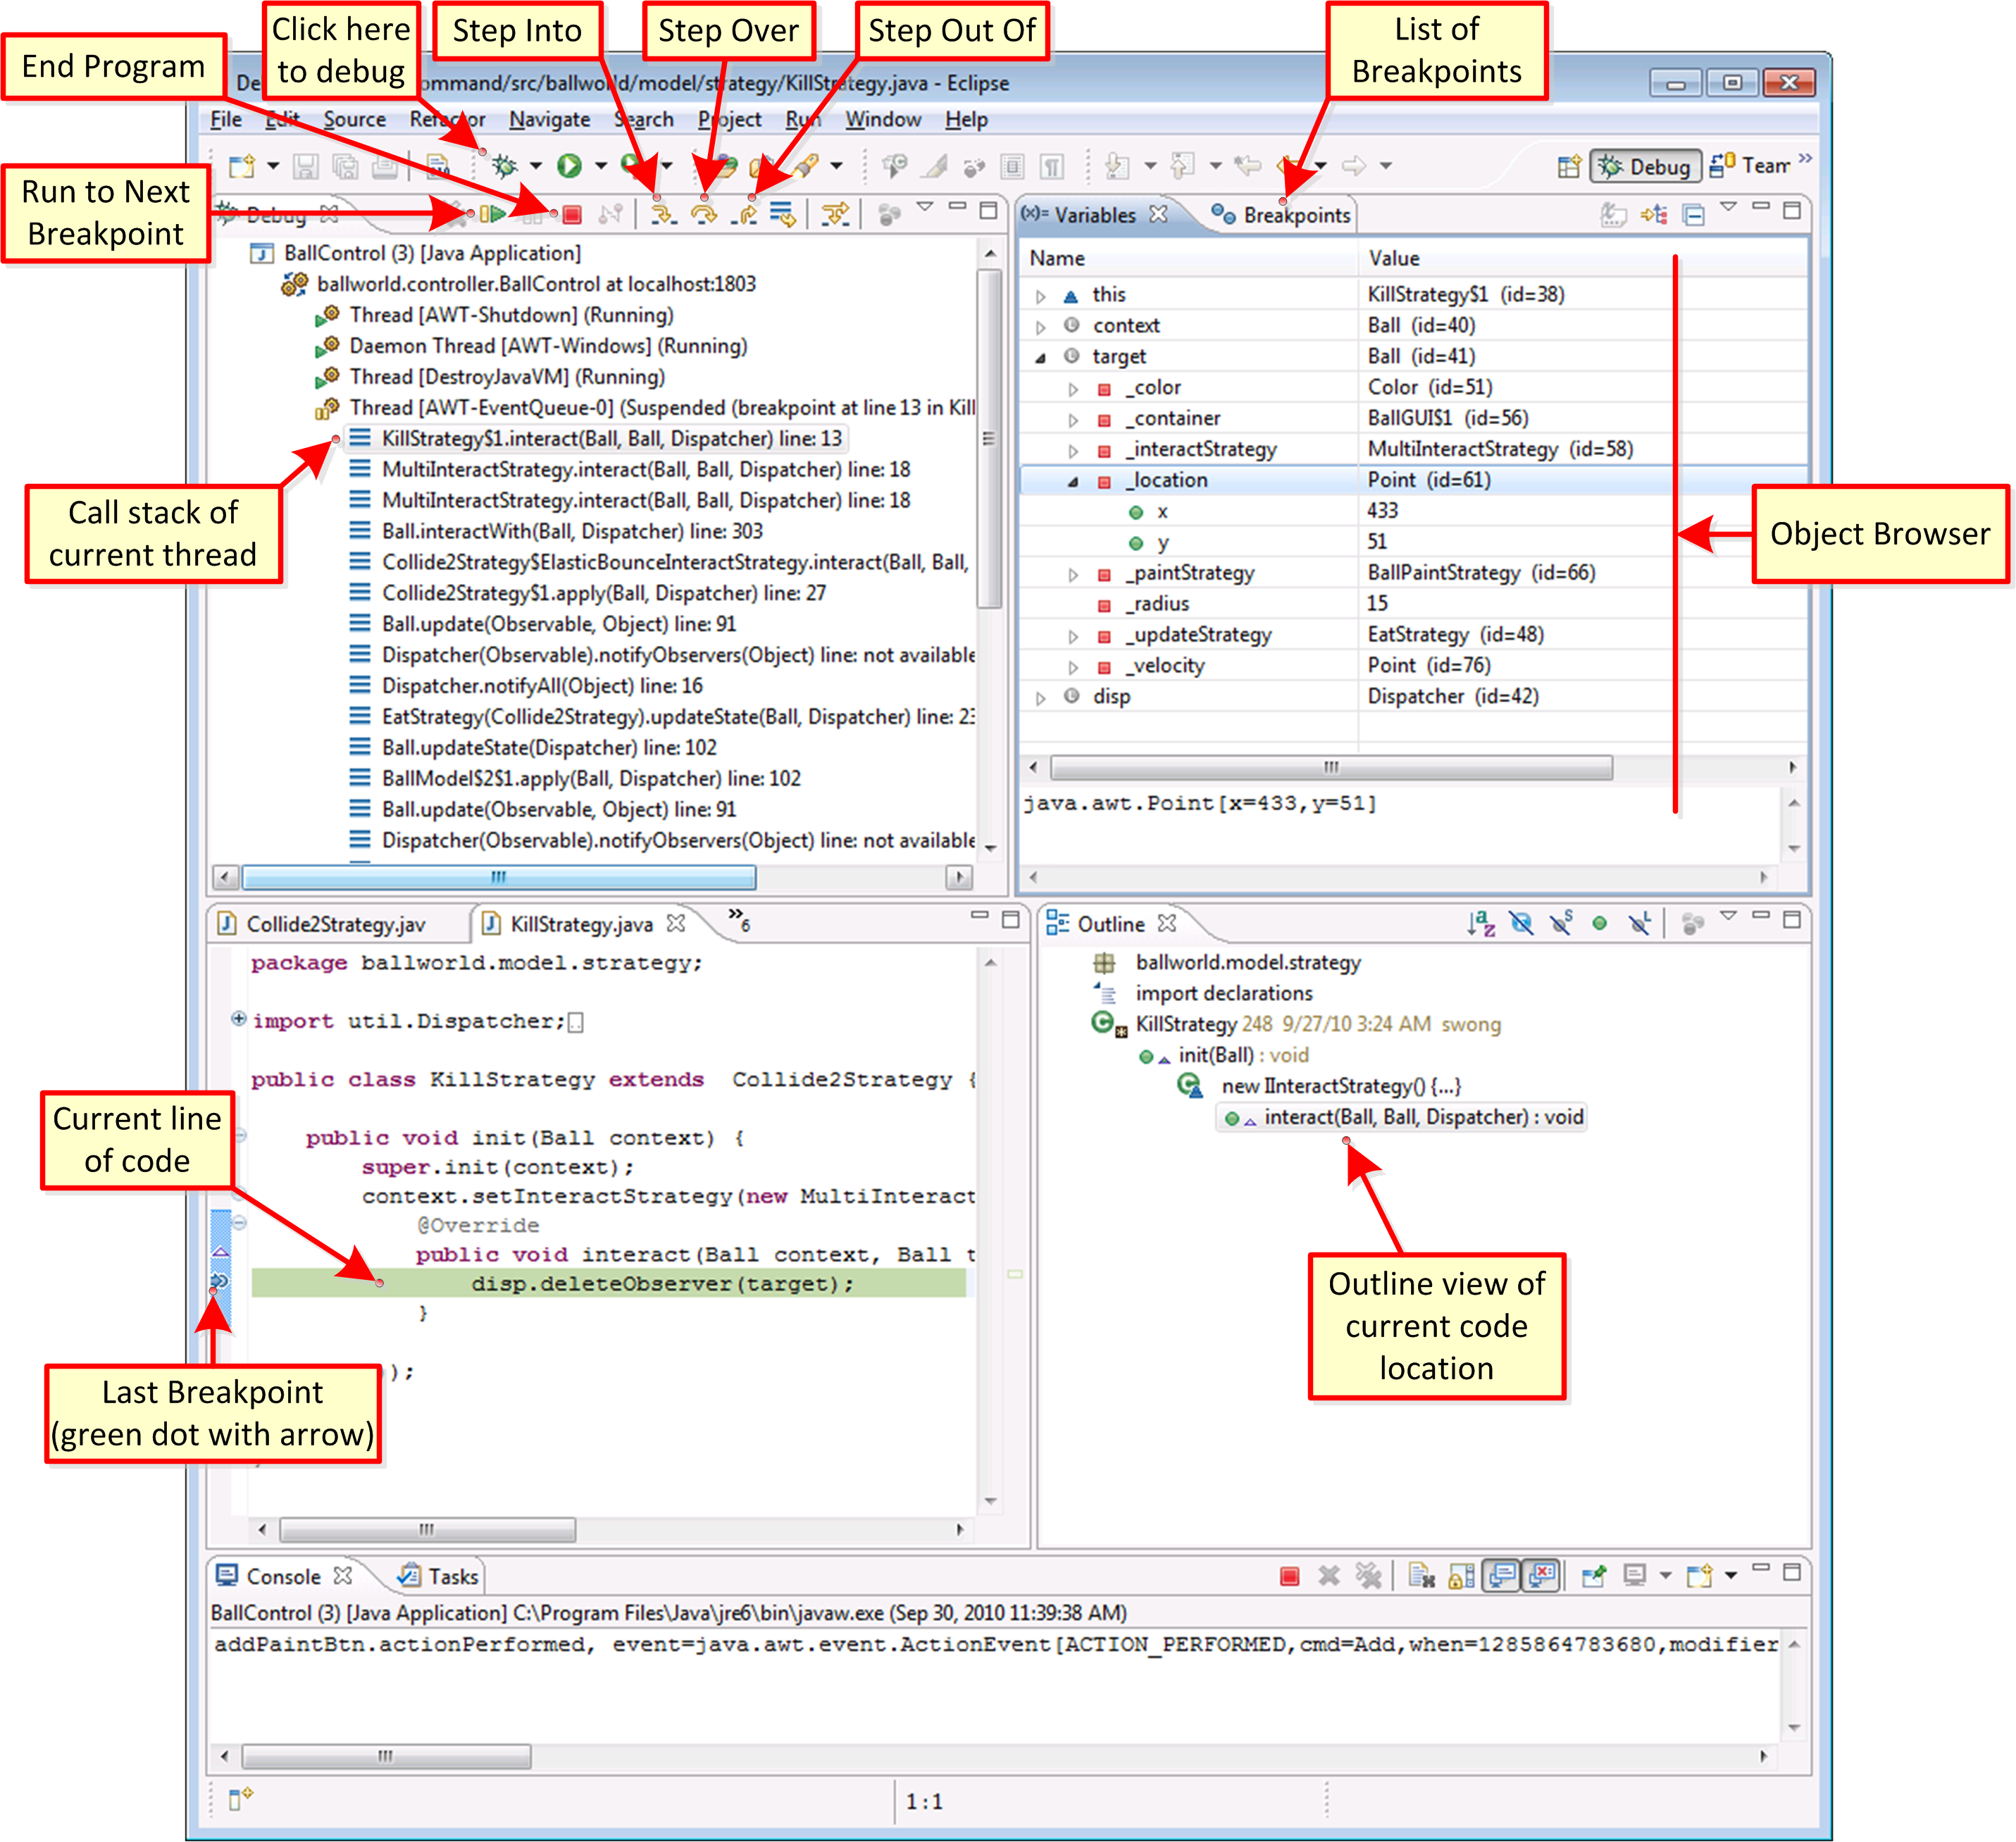
\includegraphics[width=0.7\columnwidth]{debug} 
    \bigskip
    \caption{IDE Eclipse - Debug}
\end{figure}
\bigskip
\bigskip
\section{Processo di Validazione}
Il processo di validazione è stato eseguito insieme al tutor di tirocinio \textit{Roberto Martina}. Durante gli ultimi giorni sono stati eseguiti tutti i test ed è stata confermata la validità della webapp prodotta rispetto ai requisiti definiti all'inizio dello stage. \\
Il rispetto dei canoni della struttura aziendale sono ritenuti parte fondamentale di validità del prodotto, oltre alla conformità ai requisiti. \\
Il tutor ha posto quindi molta attenzione anche su questo aspetto dato che non seguire la struttura designata portava ad un uso errato dei \textit{pattern} e dei \textit{framework} utilizzati. La struttura del codice aziendale era costruita con la consapevolezza di agevolare il programmatore nell'introduzione di nuove classi.